% Fig. 2.9 / spec Fig A08 -- the original order of the double sum
%   \sum_{x=1}^{\infty} \sum_{k=x}^{\infty} P(X=k):
%   inner sum runs rightwards along k, outer sum runs upwards along x.
% Source: mathstatch2.tex line 1255 (the tikzpicture inside the \begin{no}
%   remark of the proof of theorem `mttf`).
%
% Deviations from CH2_FIGURE_SPECS.md (all deliberate; see also the companion
% file double-sum-swapped-order.tex):
%
% 1. Spec Fig A09 asks for the two grid pictures side by side inside ONE svg.
%    NOT followed -- each picture is its own svg.  Each grid alone is about
%    7 units wide, so a side-by-side pair would be ~15 units; at the 288.6px
%    mobile display width measured for this figure the labels would then fall
%    to about 7px, far under the 12px floor of spec 1.3.  The manuscript
%    itself sets the two tikzpictures one after the other, not side by side.
%    The two files instead share one explicit bounding box (the \path below,
%    identical in both), so the axes, ticks and grid render at exactly the
%    same scale in the two svgs and can be compared row by row.
%
% 2. The manuscript separates the two sums by colour (blue inner, red outer),
%    which colour-blind readers cannot resolve.  Per spec 1.7 both are drawn
%    in journalaccent and told apart by line style: inner solid, outer dashed
%    (spec 1.7 names `on 3pt off 2pt` / `on 1pt off 2pt`; the inner one is
%    made solid instead, because the boundary line k=x is already dashed and
%    three dash patterns in one picture read as noise).  The caption must say
%    which line style is which sum.
%
% 3. The manuscript puts the outer arrow at x=7.8, giving a total width of
%    8.9 units.  It is moved to x=6.8 and shortened to 0.75--4.55 so that the
%    drawing stays inside the 9.0cm width cap of spec 1.3.  The inner sum
%    label, which the manuscript sets at (6.5,2.7), then no longer fits in the
%    strip between the arrow heads (6.4) and the outer arrow (6.8); it is
%    moved above the topmost inner arrow, where it still touches the arrow
%    family it names.
%
% 4. Type is set at 13.5pt (fix-cm makes Computer Modern scalable to that
%    size) with \DeclareMathSizes{13.5}{13.5}{11.5}{9}, instead of the 10pt
%    default with 7pt script size.  The reason is the display width: this pair
%    sits inside a proof box inside a remark box, so the figure element
%    measures 288.6px on a 390px phone and 579.7px on a 1280px desktop, not
%    the 350px / 620px a plain topic-figure--wide gets.  The smallest mark in
%    the picture is the limits on the \sum symbols, at math script size.
%
%    Native size 253.434 x 185.402 pt (drawing range 8.80cm wide, inside the
%    9.0cm cap of spec 1.3).  A mark of S pt shows at S x 0.99626 x 288.6 /
%    253.434 px, so
%        13.5pt text  -> 15.3px (mobile), 30.8px (desktop)
%        11.5pt limits-> 13.1px (mobile), 26.2px (desktop)
%    both clear of the 12px floor of spec 1.3.  At 10pt/8.5pt the same picture
%    gave 11.9px and 10.1px, i.e. under the floor.  Geometry is untouched by
%    this change: x=y=1cm as before, so the dot size, line widths, arrow heads
%    and the 0.08 gaps all keep the proportions already checked.  Any later
%    change that pushes the native width past 265pt breaks the floor again.
\documentclass[tikz,border=2pt]{standalone}
\usepackage{amsmath}
\usepackage{amssymb}
\usepackage{xcolor}
\usepackage{fix-cm}
\usetikzlibrary{arrows.meta}
\newcommand{\sssig}{\scriptscriptstyle}
\DeclareMathSizes{13.5}{13.5}{11.5}{9}

\definecolor{journalink}{HTML}{1F1C18}
\definecolor{journalmuted}{HTML}{8A7F72}
\definecolor{journalaccent}{HTML}{9C2D2D}

\begin{document}
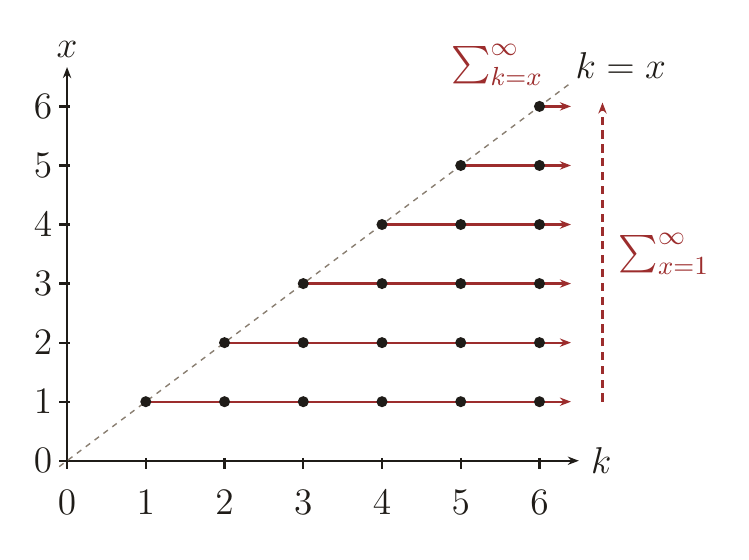
\begin{tikzpicture}[
  x=1cm,
  y=1cm,
  every node/.style={font=\fontsize{13.5}{16}\selectfont, journalink},
  axis/.style={journalink, line width=0.8pt, -{Stealth[length=4pt]}},
  tick/.style={journalink, line width=0.8pt},
  guide/.style={journalmuted, line width=0.5pt, dash pattern=on 2pt off 2pt},
  innersum/.style={journalaccent, line width=0.8pt, -{Stealth[length=4pt]}},
  outersum/.style={journalaccent, line width=0.8pt,
                   dash pattern=on 3pt off 2pt, -{Stealth[length=4pt]}},
  gridpt/.style={circle, fill=journalink, inner sep=0pt, minimum size=4pt},
  sumlab/.style={journalaccent, inner sep=0pt}
]
  % ---- common bounding box, identical in both figures of this pair ----
  \path (-0.50,-0.90) rectangle (8.30,5.50);

  % ---- axes ----
  \draw[axis] (0,0) -- (6.5,0);
  \draw[axis] (0,0) -- (0,5);
  \node[anchor=west,  inner sep=0pt] at (6.65,0) {$k$};
  \node[anchor=south, inner sep=0pt] at (0,5.12) {$x$};

  % ---- ticks on the k axis ----
  \foreach \k in {0,1,2,3,4,5,6} {
    \draw[tick] (\k,0.035) -- (\k,-0.106);
    \node[anchor=north] at (\k,-0.25) {$\k$};
  }

  % ---- ticks on the x axis (one integer step of x is 0.75 units) ----
  \foreach \y/\lab in {0.75/1, 1.5/2, 2.25/3, 3/4, 3.75/5, 4.5/6}
    \draw[tick] (0.035,\y) -- (-0.106,\y)
      node[anchor=east, inner sep=2pt] {$\lab$};
  \draw[tick] (0.035,0) -- (-0.106,0) node[anchor=east, inner sep=2pt] {$0$};

  % ---- boundary of the summation region, k = x ----
  \draw[guide] (-0.1,-0.075) -- (6.4,4.8);
  \node[anchor=south west, inner sep=1.5pt] at (6.4,4.8) {$k=x$};

  % ---- inner sum: solid, rightwards along k, from k = x to infinity ----
  \draw[innersum] (1,0.75) -- (6.4,0.75);
  \draw[innersum] (2,1.5)  -- (6.4,1.5);
  \draw[innersum] (3,2.25) -- (6.4,2.25);
  \draw[innersum] (4,3)    -- (6.4,3);
  \draw[innersum] (5,3.75) -- (6.4,3.75);
  \draw[innersum] (6,4.5)  -- (6.4,4.5);
  \node[sumlab, anchor=south east] at (6.05,4.76) {$\sum_{k=x}^{\infty}$};

  % ---- outer sum: dashed, upwards along x, from x = 1 to infinity ----
  \draw[outersum] (6.8,0.75) -- (6.8,4.55);
  \node[sumlab, anchor=west] at (7,2.625) {$\sum_{x=1}^{\infty}$};

  % ---- the lattice points, all integer pairs with k >= x (drawn last) ----
  \foreach \k in {1,2,3,4,5,6} \node[gridpt] at (\k,0.75) {};
  \foreach \k in {2,3,4,5,6}   \node[gridpt] at (\k,1.5)  {};
  \foreach \k in {3,4,5,6}     \node[gridpt] at (\k,2.25) {};
  \foreach \k in {4,5,6}       \node[gridpt] at (\k,3)    {};
  \foreach \k in {5,6}         \node[gridpt] at (\k,3.75) {};
  \node[gridpt] at (6,4.5) {};
\end{tikzpicture}
\end{document}
